\section{Results}
\label{sec:results}
We organize the results around the three predictions from Section~\ref{sec:mechanism}: whether the no-skill anchor changes a two-arm verdict, where a targeted procedure is binding rather than ceiling-limited, and whether unchanged procedures retain direction on compatible future releases. Endpoints are the independent units; repeats measure execution robustness only.

\subsection{The third arm changes the scientific verdict}
\label{sec:falsepositive}
The clearest justification for the design is a negative result. On DeepSeek C3-R cutoff, the targeted procedure succeeds on 100\% of endpoint-repeat observations and the matched generic helper on 72\%. A conventional T-versus-G comparison would therefore report a +28-point benefit. The no-skill agent, however, is also at 100\%. Thus $\widehat{\Delta}_{T-G}=+28$ points but $\widehat{\Delta}_{T-N}=0$, and Definition~1 classifies the cell as \emph{no repair}.

The frozen G1 helper explains why this is a plausible failure mode for a generic control: it validates schema-compatible evidence but is deliberately forbidden from comparing release dates with the cutoff, so it can foreground both an admissible release and a post-cutoff distractor. T1 performs the missing cutoff operation, but in this cell it only restores the behavior of the original agent. The same pattern appears more weakly in DeepSeek C4-R, while Kimi cutoff is at ceiling. The three-arm design therefore does more than reduce variance: it prevents a generic-arm deficit from being promoted into a procedure-repair claim.

A zero-call r9 audit further shows that T--G is not explained by unequal helper availability: targeted and generic helpers are each forced exactly once in all 442 retained rows of their respective arms, versus 0/442 in no-skill; condition position has no detectable success association in any arm ($p>.65$), and targeted prompts are 18.85 input tokens shorter on average than their exact generic counterparts. These diagnostics close simple invocation/order/length explanations for T--G but do not make G behaviorally neutral. We therefore execute the stronger G$_0$ control below rather than treating these diagnostics as a substitute.

\begin{figure}[t]
\centering
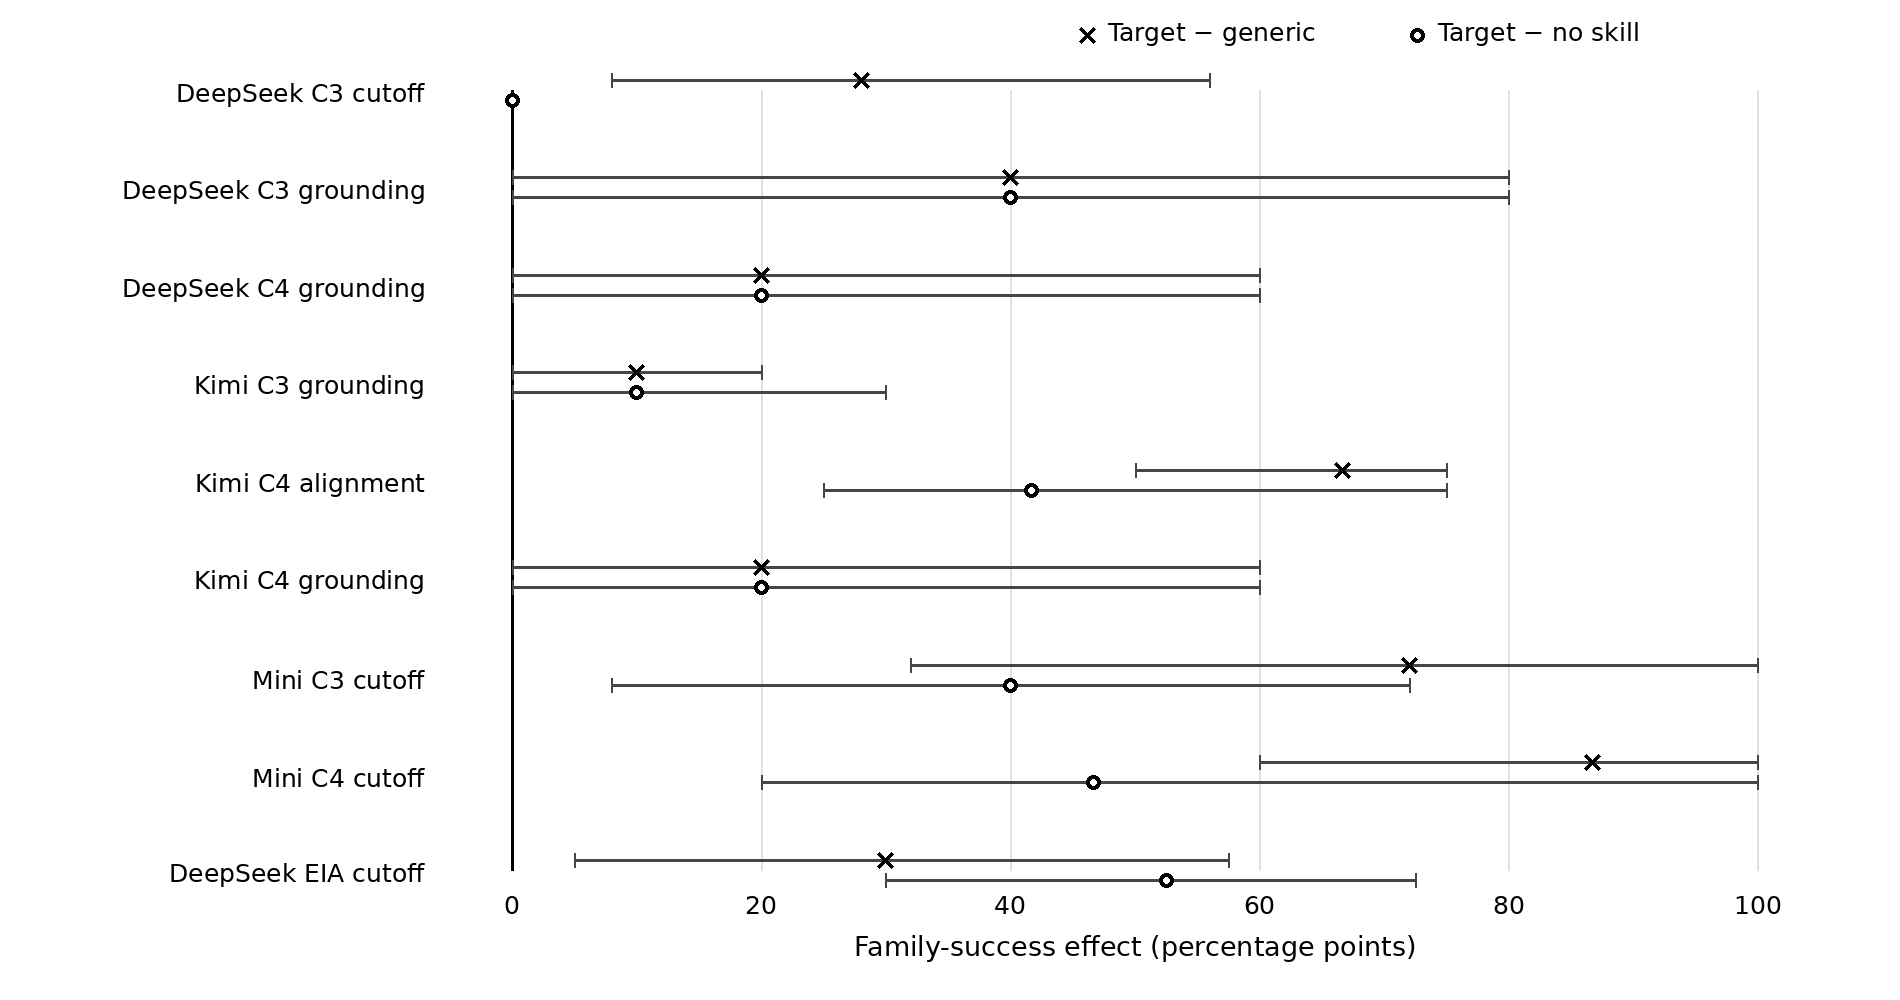
\includegraphics[width=0.96\linewidth]{figures/fig2_regime_effects.png}
\caption{Temporal-procedure effects are regime-dependent. Circles compare targeted with the original no-skill agent; crosses compare targeted with the matched generic helper. Horizontal bars show endpoint-bootstrap 95\% intervals. DeepSeek C3 cutoff illustrates the identification point: T$>$G but T$=$N, so the apparent two-arm gain is not a repair. EIA denotes the frozen post-review energy validation.}
\label{fig:regimes}
\end{figure}

The load-bearing historical cells are DeepSeek C3 grounding (20/20/60 for N/G/T), DeepSeek C4 grounding (40/40/60), and Kimi C4 alignment (58/33/100); the complete matrix, including ceiling/null cells and the later Kimi-grounding downgrade, is reported in Appendix~A.

\subsection{Stronger controls sharpen the identification boundary}
\label{sec:strongcontrols}
G$_0$ is admitted only after independent equivalence to fresh N: the frozen DeepSeek A2 replication gives G$_0$--N $=-2.1$ points, 90\% CI $[-9.3,5.0]$, and Kimi gives $+2.2$ points, CI $[-4.3,8.7]$. DeepSeek C3 grounding, C4 grounding, and held-out EIA cutoff then retain positive T--G$_0$ direction; Kimi same-domain grounding is downgraded (T--G$_0=-25$ points, T--N=0), while Kimi alignment retains +50 points over both fresh controls.

R resolves the container question. On 18 pre-frozen DeepSeek load-bearing endpoints, T--R is 0.0 points with 90\% CI $[-5.6,5.6]$ and no positive cell residual; three held-out Kimi alignment endpoints likewise give T=R=100\%. Thus the data support the operation, not a privileged callable container. Full staging and parity audits are in Appendix~A.

\subsection{Grounding is a binding repair when the original agent has headroom}
DeepSeek gives the cleanest grounding case: C3-R is 20\%/20\%/60\% for N/G/T (+40 points over both controls), and C4-R is 40\%/40\%/60\%. The fresh neutral control preserves positive direction on both pre-frozen load-bearing cells. The effect is not cross-model universal: Kimi same-domain grounding is null after G$_0$, and cross-domain grounding is also null. We therefore retain grounding as a DeepSeek-regime result rather than a general transfer claim.

\subsection{Cutoff repair appears in non-ceiling regimes and disappears at ceiling}
Cutoff effects expose the same regime boundary. The exploratory mini model has headroom on the initial replay, whereas DeepSeek C3-R is already at N ceiling. The stronger held-out EIA test freezes 12 new energy endpoints and reuses T1/G1 byte-for-byte: on eight held-out endpoints DeepSeek moves from 47.5\% (N) and 70\% (G) to 100\% (T). T--N is positive on seven of eight endpoint means (exact sign test $p=0.0156$, 95\% bootstrap interval [30,72.5] points). The mini model is instead 40/40 under N on the same EIA endpoints, so the cutoff operation is binding only when the model--task cell has headroom; the full exploratory matrix is in Appendix~A.

\subsection{Transfer is selective and explicitly bounded}
Held-out Kimi alignment moves away from ceiling historically (T/N/G=12/12, 7/12, 4/12), and the fresh control preserves T--G$_0$=T--N=+50 points on the same three endpoints. Yet operation-matched R is equally effective: T and R both succeed on all five fresh repeats. Combined with the Kimi-grounding downgrade, cross-domain grounding null, and EIA ceiling cells, transfer is selective and does not imply a uniquely effective callable surface.
